The projects presented in this chapter are proposing various ways to utilize the Ethereum blockchain as a method to ensure the integrity of cultural heritage, sensor data or provenance data for the Internet of Things (IoT). The presented projects are related to my work in terms of design goals, where the immutability and decentralization of the Ethereum blockchain replaces trusted third parties. This chapter also gives an introduction to pooled testing and a state of the art method utilized in the medical field to test a large population on COVID-19.
\section{Project Archangel}
Project ARCHANGEL is a decentralized fixity information developed in the UK with the participation of three other countries, Australia, Estonia and Norway. Their approach is to store a cryptographic hash of every incoming object of the archive on a proof-of-authority blockchain. The project started in 2017 and ended in August 2018. The goal of the project was to ensure the integrity and authenticity of digital objects in archives with the usage a private fork of the Ethereum network. Their design philosophy of operating a private blockchain has the flaw of giving a few entities the power to alter data on the blockchain. Currently, their implementation uses smart contracts as a gateway for writing to the Blockchain \cite[4]{collomosse2018archangel}.

The public's trust in Archives and Memory Institutions (AMIs) has eroded, according to the authors of the project ARCHANGEL, due to the ease with which forgery and unauthorized modifications to electronic records can be carried out due to advances in technology and the creation of numerous types of composited content. Unlike in the past, when archives relied on specific firms' products and technologies, blockchain introduces a whole new paradigm of openness and expandability. The blockchain grants permission to write records in a distributed ledger to only authorized institutions, whereas permission to view the recorded content is granted to every node participating in the blockchain. Furthermore, scalability permits the use of diverse open-source tools and the assurance of record integrity by several parties through a consensus mechanism rather than by a single centralized organization. \cite[4]{wang2021research}.
The architecture of ARCHANGEL can be seen in Figure \ref{fig:archangel} where the cryptographic hash of an incoming object is computed and then persisted onto the private blockchain. After a certain time interval, the object can be retrieved from the archived and a hash will be recomputed with the same cryptographic hash function. The object is guaranteed to be unaltered if the local and online hash value are the same.
\begin{figure}[t]
    \centering
    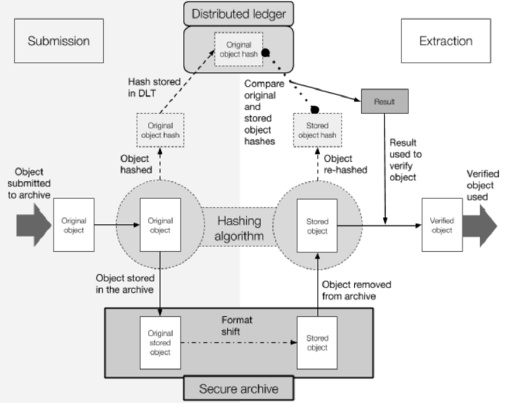
\includegraphics[width=0.5\textwidth]{archangel.png}
    \caption{Architecture of the ARCHANGEL platform \cite[2]{collomosse2018archangel}.}
    \label{fig:archangel}
\end{figure}
I agree with their vision of publicly available fixity information, where everyone with an Ethereum client is able to validate the integrity of objects in archive, but there are two points which do not conform with my vision. First and foremost is the usage of a private fork of the Ethereum network that is operated by a private set of nodes, which is basically a proof-of-authority consensus mechanism and contradicts the vision of a decentralized application \cite[3]{collomosse2018archangel}. Second, their implementation can hardly be used on the public Ethereum blockchain instead of a private fork due to the high cost of persisting data on the Ethereum main net, which is about \$8 for a SHA256 value, see Section \ref{sec:tx-cost}. 

\section{Provenance framework for the Internet of Things}
Sigwart et al. (2020) presents a data provenance framework for the IoT. Their approach is to store provenance records as so-called non-fungible assets on the Ethereum blockchain. Their prototype implements the ERC721 standard, which defines an interface for non-fungible assets or tokens (NFTs) which can be transferred by any clients (e.g., sensors, wallets), leaving a trail of provenance records created by passing the data NFT from owner to owner \cite[7]{Sigwart2020}. 
This project is important for my thesis, because it shows that the Ethereum blockchain can be utilized as a secure storage for immutable metadata which complements processes outside the blockchain.
Contrary to their implementation, I decided to not utilize the ERC721 standard since the data in my case, fixity information, does not need to be transferred from owner to owner. In order to use their implementation for fixity information instead of provenance data, you would have to deploy or "mint" an NFT for each digital object in the archive. That means, massive overhead in operation cost since "minting" is basically a deployment of a smart contract, which is one of the most expensive operations on the Ethereum blockchain, see Table \ref{table:gas-costs}.

\section{Remote Data Integrity Checking Scheme}
Zhao et al. (2020) presents a blockchain based remote data integrity checking scheme. Their scheme consists of three phases, including setup, storage and verification phase. This scheme may be of great importance for my work because it integrates well with the work of Sigwart et al. (2020) in terms of design goals. The detail of each phase in their scheme is described as follows: (1) Setup phase, where the public key is uploaded to the blockchain. (2) Storage phase, where the data owner signs the data blocks and uploads them to a cloud storage. (3) Verification phase, where the data owner downloads the data or desires to check the integrity of the individual data. The auditing process is done by verifying the signature of the data blocks by the data owner \cite[1]{zhao2020blockchain}.
The remote data integrity checking scheme utilizes the blockchain as a method to validate the integrity of IoT information management systems without involving trusted third parties, whereas the projects presented before utilizes the blockchain as a metadata storage.


\section{Pooled testing}\label{sec:pooled}
Pooled Testing was first introduced by \cite{dorfman1943detection} as a strategy to screen numerous military recruits for syphilis during World War 2. Dorfman envisioned that instead of testing each recruit's blood specimen separately, multiple specimens could be pooled together and tested at once. Positive pools' specimens would be retested individually to determine which recruits had contracted the disease, whereas negative pools' specimens would be declared negative. Dorfman wanted to save money on testing while still identifying all syphilitic-positive candidates, so he used group testing. Because the goal is to identify all positive persons among all individuals tested, this is now known as the "case identification problem." Dorfman's case identification method can be thought of as a two-stage hierarchical algorithm. Individuals from positive pools are tested in the second stage after non-overlapping pools have been screened in the first.

In this thesis, two strategies of pooled testing are implemented. 
First, two stage hierarchical pooling strategy, where in the first stage of this protocol N pools get initialized and filled with samples of the population. If the combined result of the pool is negative than no second stage is needed, but when a pool is declared positive a second stage is needed and all individuals from this pool have to be retested in order to find the corrupted individual. The expected number of test is equal to the number of tests in the first stage added to the number of tests in the second stage \cite[3]{nianogo2021optimal}.
The second strategy is context-sensitive pooling, where homogeneous samples are grouped in order to separate groups with different change rates. Hence, if one member of a pooled group is corrupted, there is a high likelihood that other group members are also corrupted \cite[3]{deckert2020simulation}.

\section{Summary}
The blockchain related projects presented in this chapter have a common vision, which is a decentralized storage for metadata to validate the integrity and authenticity of data used in applications. The ability for the public to validate that an authority did not tamper with the data in their care is important and the removal of trust strengthens the trust in public institutions. More on the subject of trust can be seen in Chapter \ref{ch:diplomatics}
Decentralization and trust aside, the cost of the fixity storage presented in this thesis is also more than relevant as later seen in Chapter \ref{ch:ethereum}, where the cost and computational effort of interacting with the Ethereum network is presented.
